\section{Background}
We regard an image $I$ as a function that maps voxels of a rectangular grid \hbox{$\mathcal{L}$}, of dimensions $n_{x} \times n_{y} \times n_{z}$ cells, to a set $G$ of
possible values called the ``dynamic range'' of $I$. The images we are interested in represent objects in physical space. This means that each point $(i,j,k)$ in the
3-dimensional grid $\mathcal{L}$ is associated to a point $(x,y,z) \in \Omega \subset \mathbf{R}^{3}$. The function that maps voxel coordinates of a grid $\mathcal{L}$ to their corresponding coordinates in physical space is an invertible affine transformation. From now on, we implicitly assume that any grid $\mathcal{L}$ is associated with a specific grid-to-space affine transformation. Since the grid-to-space transformation is invertible, we can, and will, unambiguously talk about images defined in physical space $\Omega \subset \mathbf{R}^{3}$.\\
%Since our images represent objects in physical space, and these objects are not tied to any specific grid, the same object may be sampled over any grid $\mathcal{L}$.

\vspace{-0.5cm}
\subsection{Non-linear image registration}\label{sec:non_linear_image_registration}
The goal of image registration is to compute a transformation $\phi: \Omega_{I} \rightarrow \Omega_{J}$ that brings a moving image $J:\Omega_{J} \rightarrow G$ into correspondence
with a fixed image $I:\Omega_{I} \rightarrow G$. Correspondence between $I$ and $J$ is defined to be reached when a matching functional measuring the dissimilarity between them is minimized. In non-linear image registration, the transformation $\phi$ is usually represented by a deformation field $\mathbf{u(\cdot)}$ that assigns a displacement vector
to each point $x$ such that $\phi(x) = x + \mathbf{u}(x)$. The classical elastic model is one of the earliest formulation for non-linear image registration \cite{Bajcsy1982, Gee1999}, and may be written as
\begin{equation}\label{eq:elastic}
    \mathbf{u}^{*} = \arg \min_{\mathbf{u}} \int_{\Omega} ||L \mathbf{u}(x)||^{2}dx + \Pi(I, J \circ \phi),
\end{equation}
where $L$ is a differential operator used to promote smoothness on $\mathbf{u}$ and $\Pi$ is the dissimilarity metric driving the registration. A limitation of this model, especially important for medical image registration is that the solution, although being smooth, is not guaranteed to be invertible, and the topology of the moving image is not guaranteed to be preserved after transforming it under $\phi$.\\

%Beg's Large Deformation Diffeomorphic Metric Mapping (LDDMM) \cite{Science2005} formulation of the registration problem is given by:
%\begin{equation}\label{eq:LDDMM}
%    v^{*} = \arg \min_{v:\dot{\phi} = v_{t}(\phi)} \int_{0}^{1} ||L v_{t}||^{2} dt + \Pi(I, J \circ \phi(\cdot, 1)),
%\end{equation}
%where $\dot{\phi} = \frac{d\phi}{dt}$, $v_{t} = v(\cdot, t), t\in [0, 1]$. The final diffeomorphisms can be obtained by integrating over time
%\begin{equation}\label{eq:velocity_integral}
%    \phi(x, 1) = \phi(x, 0) + \int_{0}^{1}v(\phi(x, t), t) dt.
%\end{equation}
%This and other formulations also based on diffeomorphic flows ensure that images are smoothly transformed and their topology preserved: an important property for many medical %applications.
To overcome the limitations of the elastic model, the large deformation model proposed by Christensen {\it et al.} \cite{Christensen2001} and further developed by Beg {\it et al.} \cite{Science2005} formulates the problem in terms of a trajectory of transformations \hbox{$\phi:\Omega_{I} \times [0, 1] \rightarrow \Omega_{J}$} that satisfies $\frac{d \phi(x, t)}{dt} = v(\phi(x, t), t)$ and $\phi(x, 0) = x$, where $v(\cdot, \cdot)$ is the velocity field associated to the curve $\phi$. Dupuis {\it et al.} \cite{Dupuis1998} showed that by enforcing sufficient smoothness in $v$, through the differential operator $L$, it can be guaranteed that $\phi(\cdot, t), t \in [0, 1]$ are diffeomorphisms. Avants {\it et al.} \cite{Avants2008, Avants2011} modified the standard large deformation model to enforce symmetry in the sense that the registration result is the same regardless of which image we designate as $I$ and $J$. By splitting the trajectory $\phi$ into two trajectories with opposite direction $\phi_{1}(x, t) = \phi_{2}(y, 1-t)$, where $y = \phi(x, 1)$, with corresponding velocity fields $v_{1}, v_{2}$, the Symmetric formulation for Diffeomorphic Image Registration \cite{Avants2008, Avants2011} can be written as:
\begin{equation}\label{eq:syn_energy}
    \begin{array}{lll}
        v_{1}^{*}, v_{2}^{*} &=& \mathlarger{\arg \min \int_{t=0}^{0.5} ||L v_{1}(x, t)||^{2} + ||L v_{2}(x, t)||^{2} dt}\\
        &+& \mathlarger{ \Pi(I \circ \phi_{1}(\cdot, 0.5), J(\phi_{2}(\cdot, 0.5)))}
    \end{array}
\end{equation}
subject to
\begin{equation}\label{eq:syn_energy_constraints}
    \begin{array}{l}
        \frac{d\phi_{i}(x, t)}{dt} = v_{i}(\phi(x,t),t)\\
        \phi_{i}(\cdot, 0) = \mathbf{I},\, \phi_{i}^{-1}(\phi_{i}) = \mathbf{I},\, \phi_{i}(\phi_{i}^{-1}) = \mathbf{I},\, i=1,2,
    \end{array}
\end{equation}
where $\mathbf{I}$ denotes the identity transformation. Avants {\it et al.} \cite{Avants2006} proposed a numerical algorithm, called \textit{Geodesic SyN} for solving \eqref{eq:syn_energy}, which deforms both images towards the midpoint of the trajectory. The main drawback of directly solving \eqref{eq:syn_energy} is its computational cost, since it requires space and time discretization and it is necessary to integrate the velocity fields at each iteration to obtain the trajectories. A more efficient optimization algorithm to approximately solve \eqref{eq:syn_energy}, also proposed by Avants {\it et al.} \cite{Avants2008, Avants2011}, consists in computing the gradient of the metric only at the midpoint of the trajectory:
\begin{equation}\label{eq:grad_metric}
    \nabla_{\phi_{i}} \Pi(\tilde{I}, \tilde{J}) = \frac{\partial}{\partial \phi_{i}} \Pi \left( \tilde{I}, \tilde{J}\right),
\end{equation}
where $\tilde{I} = I \circ \phi_{1}^{-1}(\cdot, 0.5)$, $\tilde{J} = J \circ \phi_{2}^{-1}(\cdot, 0.5)$. The midpoint diffeomorphisms are then updated by composition with the gradient after smoothing with a Gaussian kernel $K_{\sigma}$:
\begin{equation}\label{eq:gsyn_update}
    \phi_{i}(\cdot, 0.5) = \phi_{i}(\cdot, 0.5) - \left( \epsilon K_{\sigma} \ast \nabla_{\phi_{i}} \Pi(\tilde{I}, \tilde{J}) \right) \circ \phi_{i}(\cdot, 0.5),
\end{equation}
where $\ast$ denotes the convolution operator and $\epsilon$ is a small factor controlling the step size in the optimization process. Finally, the updated midpoint transformations (which, after composition with the gradient, are not ensured to be diffeomorphisms) are forced to be invertible by using an explicit vector field inversion algorithm \cite{Chen2008}. This algorithm, called \textit{Greedy SyN} (alg. \ref{alg:Greedy_SyN}) has been adopted by the neuroimaging community as the \textit{de facto} state-of-the-art brain MRI registration algorithm due to its reliability and efficiency. It was the method used for evaluating ANTS \cite{Avants2011} in the large comparative studies performed by Klein {\it et al.} \cite{Klein2009, Klein2010} in which \textit{Greedy SyN} was consistently ranked among the top performers.

\begin{algorithm}[h!]
\caption{{\small Greedy SyN (available in ANTS \cite{Avants2011}). This algorithm was consistently ranked among the top performers in the large comparative studies performed by Klein {\it et al.} \cite{Klein2009, Klein2010}.}}\label{alg:Greedy_SyN}
\begin{algorithmic}[1]
\REQUIRE Gaussian kernel parameter $\sigma>0$
\REQUIRE Step size $\epsilon>0$
\REQUIRE Maximum number of iterations $T>0$
\STATE Initialize: $\phi_{i}(\cdot, 0.5) = Id, i=1, 2$
\STATE $t=0$
\REPEAT
    \STATE Warp $\tilde{I}  = I \circ \phi_{1}^{-1}(\cdot, 0.5), \tilde{J} = J \circ \phi_{2}^{-1}(\cdot, 0.5)$
    \STATE Compute the gradients $\mathbf{u}_{i} = \nabla_{\phi_{i}} \Pi(\tilde{I}, \tilde{J}), i=1,2$
%    \STATE Update $\phi_{i}(\cdot, 0.5), i=1, 2$ according to \eqref{eq:gsyn_update}
    \STATE Update $\phi_{i}(\cdot, 0.5) = \phi_{i}(\cdot, 0.5) - \left( \epsilon K_{\sigma} \ast \mathbf{u}_{i} \right) \circ \phi_{i}(\cdot, 0.5)$
    \STATE Invert $\phi_{i}^{-1}(\cdot, 0.5) = invert (\phi_{i}(\cdot, 0.5)), i=1, 2$
    \STATE Invert $\phi_{i}(\cdot, 0.5) = invert (\phi_{i}^{-1}(\cdot, 0.5)), i=1, 2$
    \STATE t = t + 1
\UNTIL{$t\geq T$ or convergence}
\RETURN $\phi_{i}(\cdot, 0.5), i=1,2$
\end{algorithmic}
\end{algorithm}\figcloser

\subsection{Local linear reconstruction}
Defining an adequate matching functional is arguably the most important aspect of image registration, and has been the subject of significant amount of research \cite{Sotiras2013}. In the mono-modal case, a plausible model relating the input images $I$ and $J$ by means of the (unknown) transform $\phi$ is given by
\begin{equation}\label{eq:ssd_model}
    I(v) = J(\phi(v)) + \eta(v), \; \forall v\in\Omega_{I}
\end{equation}
where the Gaussian random variables $\eta(v) \sim N(0, \sigma^{2})$ are assumed to be independent and identically distributed. Under these assumptions, the negative log-likelihood of the observed images is proportional to the Sum of Squared Differences (SSD), given by
\begin{equation}\label{eq:ssd_functional}
    SSD(I, J; \phi) = \sum_{v \in \Omega_{I}} \left(I(v) - J(\phi(v))\right)^{2}.
\end{equation}
Thus, minimization of \eqref{eq:ssd_functional} with respect to the transformation $\phi$ corresponds to a maximum likelihood estimation (m.l.e.) of the parameters of model \eqref{eq:ssd_model} (the parameters being the transformation $\phi$). There are two main limitations of model \eqref{eq:ssd_model} in the context of brain MRI: a) it does not take into account spatial intensity inhomogeneities and b) the functional is computed \emph{point-wise}, which makes it susceptible to noise and unable to capture the local structure of the images \cite{Heinrich2012}. To overcome these limitations, Wang and Pan \cite{Wang2014} recently proposed a local linear model that attempts to account for the bias field in brain MRI. Let $W_{v} = \left\lbrace v_{1}, v_{2}, ..., v_{n} \right\rbrace$ be a rectangular local window centered at $v\in\Omega_{I}$, containing $n$ points and denote by $\mathbf{x}_{v} = (I(v_{1}), I(v_{2}), ..., I(v_{n}))^{T}$, $\mathbf{y}_{v} = (J(\phi(v_{1})), J(\phi(v_{2})), ..., J(\phi(v_{n})))^{T}$ the input images evaluated at all points $v_{i}\in W_{v}$, $i=1, ..., n$. Please keep in mind that $\left\lbrace\mathbf{x}_{v}\right\rbrace$ are fixed (they never change during optimization) while $\left\lbrace\mathbf{y}_{v}\right\rbrace$ change as we move $\phi$. Wang's local linear model states that, when $\phi$ correctly aligns $J$ to $I$, their intensities are approximately locally linear:
\begin{equation}\label{eq:wang_model}
    \mathbf{y}_{v} = \left[\mathbf{x}_{v} \; \mathbbm{1}\right]\beta + \eta(v) \; \forall v\in\Omega_{I}
\end{equation}
where $\mathbbm{1}$ is an $n$-vector whose entries are all equal to $1$,  $\beta = (\beta_{0}, \beta_{1})^{T}$ is the vector of $2$ parameters of the local linear model and the random vectors $\eta(v)\sim N(0, \sigma^{2} \mathbbm{I}_{n})$ are assumed to be independent and identically distributed, where $\mathbbm{I}_{n}$ is the $n \times n$ identity matrix. It is important to notice that independence is a typical assumption to make the inference more tractable. However, since local windows overlap, the random vectors are not independent in general. The m.l.e. for $\beta$ can be directly computed as
\begin{equation}\label{eq:wang_model_mle_beta}
    \widehat{\beta} =
    \left[\begin{array}{cc}
        \mathbf{x}_{v}^{T}\mathbf{x}_{v} & \mathbf{x}_{v}^{T}\mathbbm{1}\\
        \mathbf{x}_{v}^{T}\mathbbm{1} & n
    \end{array}\right]^{-1}
    \left[\begin{array}{c}
        \mathbf{x}_{v}^{T}\\
        \mathbbm{1}^{T}
    \end{array}\right]\mathbf{y}_{v}.
\end{equation}
By substituting $\beta = \widehat{\beta}$ in \eqref{eq:wang_model}, and summing over all points $v\in\Omega_{I}$ the negative log-likelihood is proportional to the ``local linear reconstruction'' (LLR) matching functional, proposed by Wang and Pan \cite{Wang2014}:
\begin{equation}\label{eq:wang_metric}
    LLR(I, J;\phi) = \sum_{v\in\Omega_{I}}|| (\mathbf{Q}_{v} - \mathbbm{I}_{n})\mathbf{y}_{v}||^{2},
\end{equation}
\vspace{-0.2cm}
where
\vspace{-0.2cm}
\begin{equation}\label{eq:def_P_v}
    \mathbf{Q_v} = [\mathbf{x}_{v} \; \mathbbm{1}]
    \left[\begin{array}{cc}
        \mathbf{x}_{v}^{T}\mathbf{x}_{v} & \mathbf{x}_{v}^{T}\mathbbm{1}\\
        \mathbf{x}_{v}^{T}\mathbbm{1} & n
    \end{array}\right]^{-1}
    \left[\begin{array}{c}
        \mathbf{x}_{v}^{T}\\
        \mathbbm{1}^{T}
    \end{array}\right].
\end{equation}
The LLR matching functional turns out to be very robust for mono-modal registration. However, in some multi-modal registration tasks, the local linear model is insufficient to describe the relationship between image modalities. To exemplify this, Fig. \ref{fig:llr_test} depicts an example of the residual error of local linear reconstructions between two aligned brain images\footnote{See supplementary material for an enlarged version of Fig. \ref{fig:llr_test}.} (a T1 and a T2 image) from the Brainweb \cite{Cocosco1997} dataset\footnote{The Brainweb dataset was used by Wang and Pan \cite{Wang2014} in their evaluations.}. The center image in Fig. \ref{fig:llr_test} depicts the reconstruction error in false color. Although the local relationship between both images is close to linear almost everywhere, there are local regions where the intensity relationship is not close to linear regardless of what image is selected as predictor.\\

%\begin{figure}[t!]
%\centering
%    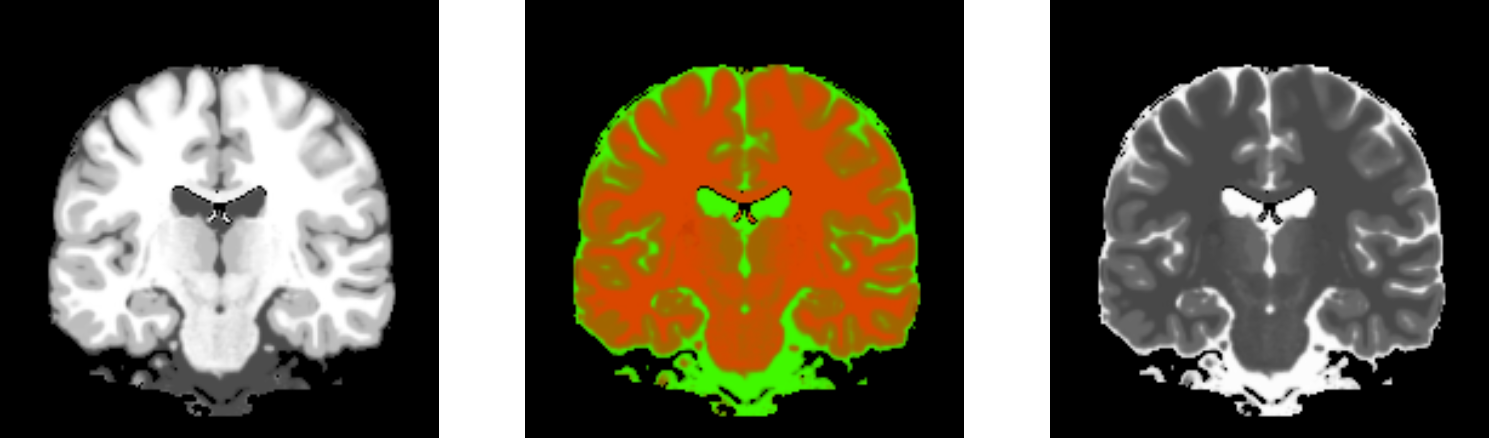
\includegraphics[width=1.0\linewidth]{./images/brainweb_t1_t2_overlay.png}\\
%    \caption{{\small Coronal slice of two realistic brain MR images from the Brainweb \cite{Cocosco1997} dataset. The center image is an overlay of the T1 (left) image in the red %channel, over the T2 (right) image in the green channel.}}
%\label{fig:brainweb_t1_t2}\figcloser
%\end{figure}

%Note: coordinates of selected windows: (125, 108, 31) and (50, 108, 67)
\begin{figure}[t!]
\centering
    \subfloat[]{\label{fig:T1T2_affine_fit_scatter1}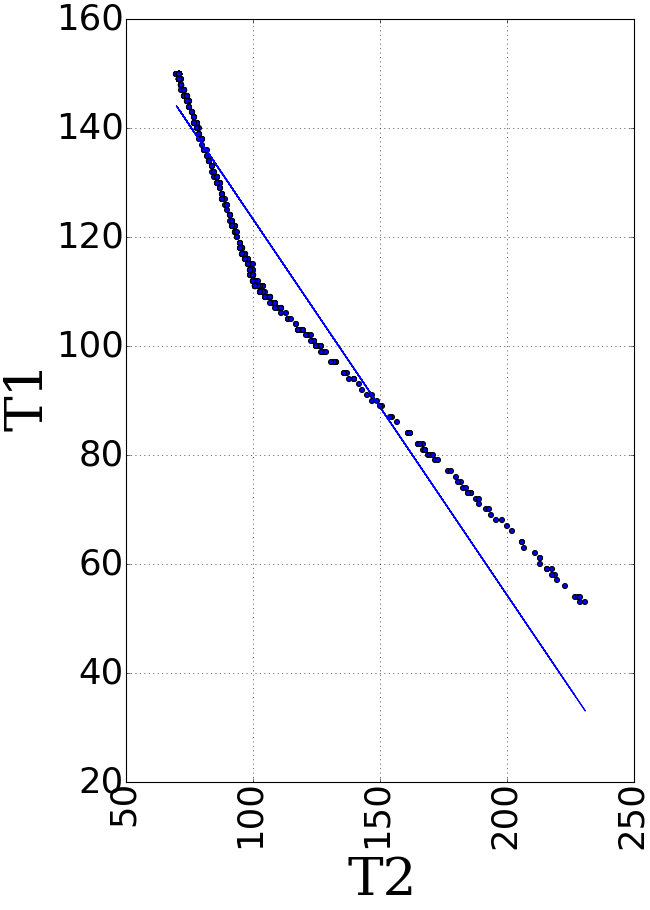
\includegraphics[width=0.2\linewidth]{./images/t1_aafo_t2_sample2_lt.png}}
    \subfloat[]{\label{fig:T1T2_affine_fit_scatter2}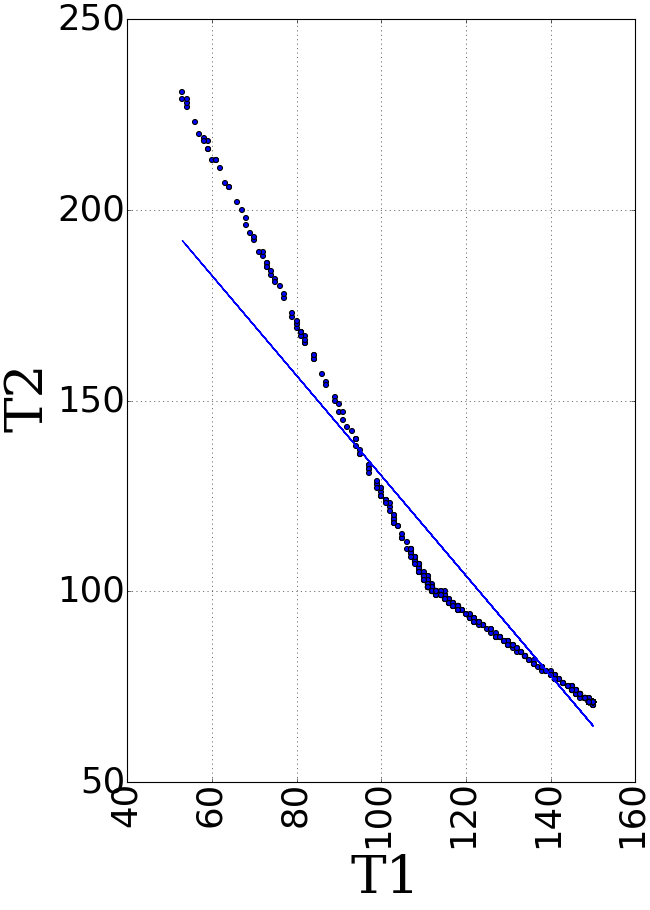
\includegraphics[width=0.2\linewidth]{./images/t2_aafo_t1_sample2_lt.png}}
    \subfloat[]{\label{fig:T1T2_affine_fit_map}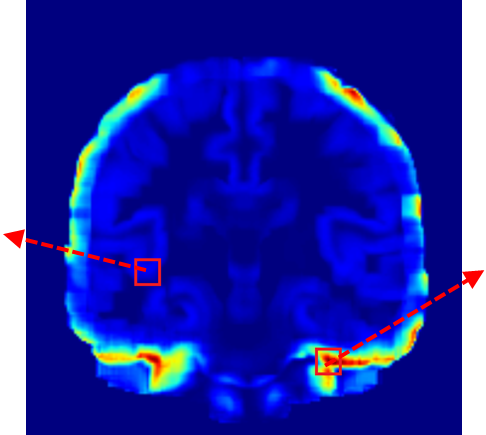
\includegraphics[width=0.2\linewidth]{./images/residuals_input_arrows.png}}
    \subfloat[]{\label{fig:T1T2_affine_fit_scatter1}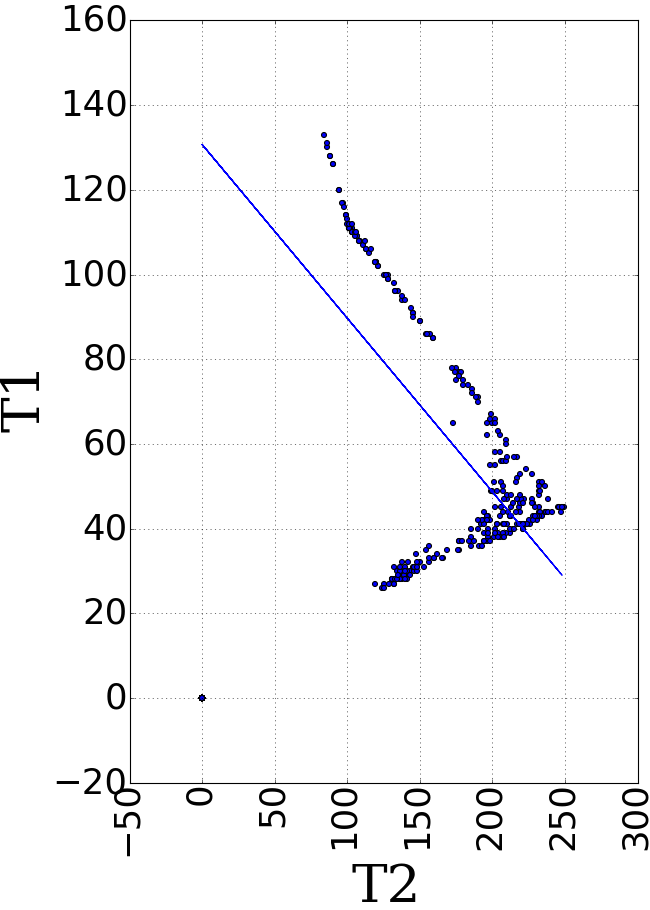
\includegraphics[width=0.2\linewidth]{./images/t1_aafo_t2_sample1_lt.png}}
    \subfloat[]{\label{fig:T1T2_affine_fit_scatter2}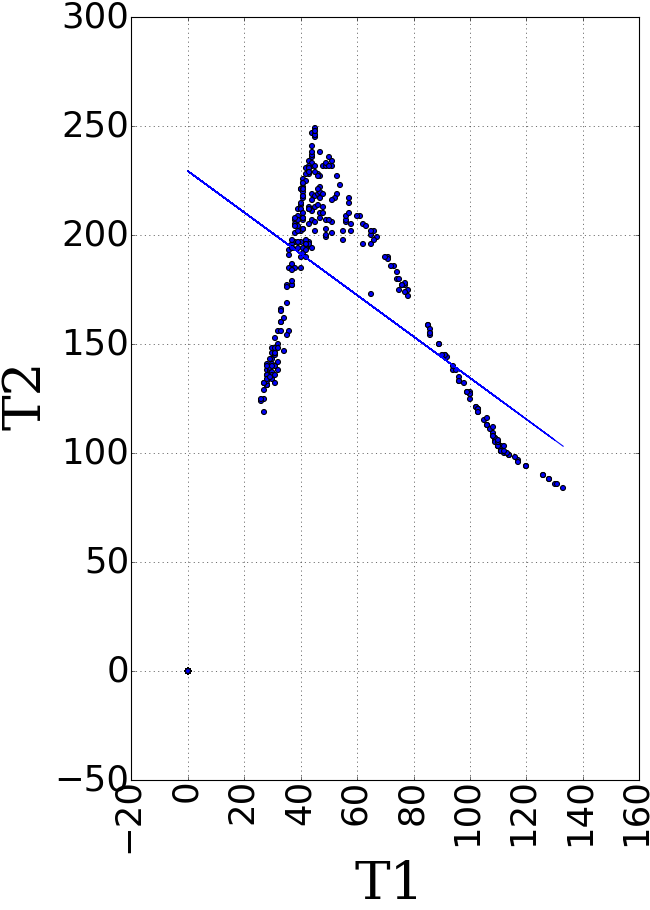
\includegraphics[width=0.2\linewidth]{./images/t2_aafo_t1_sample1_lt.png}}\\
    \caption{{\small Local linear reconstruction between T1 and T2 images under perfect alignment. Center image (c) depicts the reconstruction error in false color. Two local windows were selected: Left (a, b): a local window with a close-to-linear relationship. Right (d, e): a local window with a far from linear relationship. The scatter plots depict the best affine fit of T1 intensities as a function of T2 (a, d), and the best fit of T2 as a function of T1 (b, e).}}
\label{fig:llr_test}\figcloser
\end{figure}





